\vspsec
\section{Introduction}
\vspsec
Both model-based and model-free reinforcement learning (RL) methods generally operate in one of two regimes: all training is performed in advance, producing a model or policy that can be used at test-time to make decisions in settings that approximately match those seen during training; or, training is performed online (e.g., as in the case of online temporal-difference learning), in which case the agent can slowly modify its behavior as it interacts with the environment. However, in both of these cases, dynamic changes such as failure of a robot's components, encountering a new terrain, environmental factors such as lighting and wind, or other unexpected perturbations, can cause the agent to fail. In contrast, humans can rapidly adapt their behavior to unseen physical perturbations and changes in their dynamics~\citep{braun2009learning}: adults can learn to walk on crutches in just a few seconds, people can adapt almost instantaneously to picking up an object that is unexpectedly heavy, and children that can walk on carpet and grass can quickly figure out how to walk on ice without having to relearn how to walk. How is this possible? If an agent has encountered a large number of perturbations in the past, it can in principle use that experience to \emph{learn how to adapt}. In this work, we
propose a meta-learning approach for learning online adaptation.

Motivated by the ability to tackle real-world applications, we specifically develop a model-based meta-reinforcement learning algorithm. In this setting, data for updating the model is readily available at every timestep in the form of recent experiences. But more crucially, the meta-training process for training such an adaptive model can be much more sample efficient than model-free meta-RL approaches~\citep{duan2016rl2,wang2016learning,finn2017maml}. Further, our approach foregoes the episodic framework on which model-free meta-RL approaches rely on, where tasks are pre-defined to be different rewards or environments, and tasks exist at the trajectory level only. Instead, our method considers each timestep to potentially be a new ``task, " where any detail or setting could have changed at any timestep. This view induces a more general meta-RL problem setting by allowing the notion of a task to represent anything from existing in a different part of the state space, to experiencing disturbances, or attempting to achieve a new goal.

Learning to adapt a model alleviates a central challenge of model-based reinforcement learning: the problem of acquiring a global model that is accurate throughout the entire state space. Furthermore, even if it were practical to train a globally accurate dynamics model, the dynamics inherently change as a function of uncontrollable and often unobservable environmental factors, such as those mentioned above. If we have a model that can adapt online, it need not be perfect everywhere a priori. This property has previously been exploited by adaptive control methods~\citep{aastrom2013adaptive,sastry1989adaptive, pastor2011online, franzi2016robustonline}; but, scaling such methods to complex tasks and nonlinear systems is exceptionally difficult. Even when working with deep neural networks, which have been used to model complex nonlinear systems~\citep{thanard}, it is exceptionally difficult to enable adaptation, since such models typically require large amounts of data and many gradient steps to learn effectively. By specifically training a neural network model to require only a small amount of experience to adapt, we can enable effective online adaptation in complex environments while putting less pressure on needing a perfect global model. 

The primary contribution of our work is an efficient meta reinforcement learning approach that achieves online adaptation in dynamic environments. To the best knowledge of the authors, this is the first meta-reinforcement learning algorithm to be applied in a real robotic system. Our algorithm efficiently trains a global model that is capable to use its recent experiences to quickly adapt, achieving fast online adaptation in dynamic environments. We evaluate two versions of our approach, recurrence-based adaptive learner (ReBAL) and gradient-based adaptive learner (GrBAL) on stochastic and simulated continuous control tasks with complex contact dynamics (Fig.~\ref{fig:mujoco-envs}). In our experiments, we show a quadrupedal ``ant'' adapting to the failure of different legs, as well as a ``half-cheetah" robot adapting to the failure off different joints, navigating terrains with different slopes, and walking on floating platforms of varying buoyancy. Our model-based meta RL method attains substantial improvement over prior approaches, including standard model-based methods, online model-adaptive methods, model-free methods, and prior meta-reinforcement learning methods, when trained with similar amounts of data. In all experiments, meta-training across multiple tasks is sample efficient, using only the equivalent of $1.5-3$ hours of real-world experience, roughly $10\times$ less than what model-free methods require to learn a single task. Finally, we demonstrate GrBAL on a real dynamic legged millirobot (see Fig~\ref{fig:mujoco-envs}). To highlight not only the sample efficiency of our meta model-based reinforcement learning approach, but also the importance of fast online adaptation in the real world, we show the agent's learned ability to adapt online to tasks such as a missing leg, novel terrains and slopes, miscalibration or errors in pose estimation, and new payloads to be pulled. 
\begin{figure}[t]
\vspace{-0.2cm}
\centering
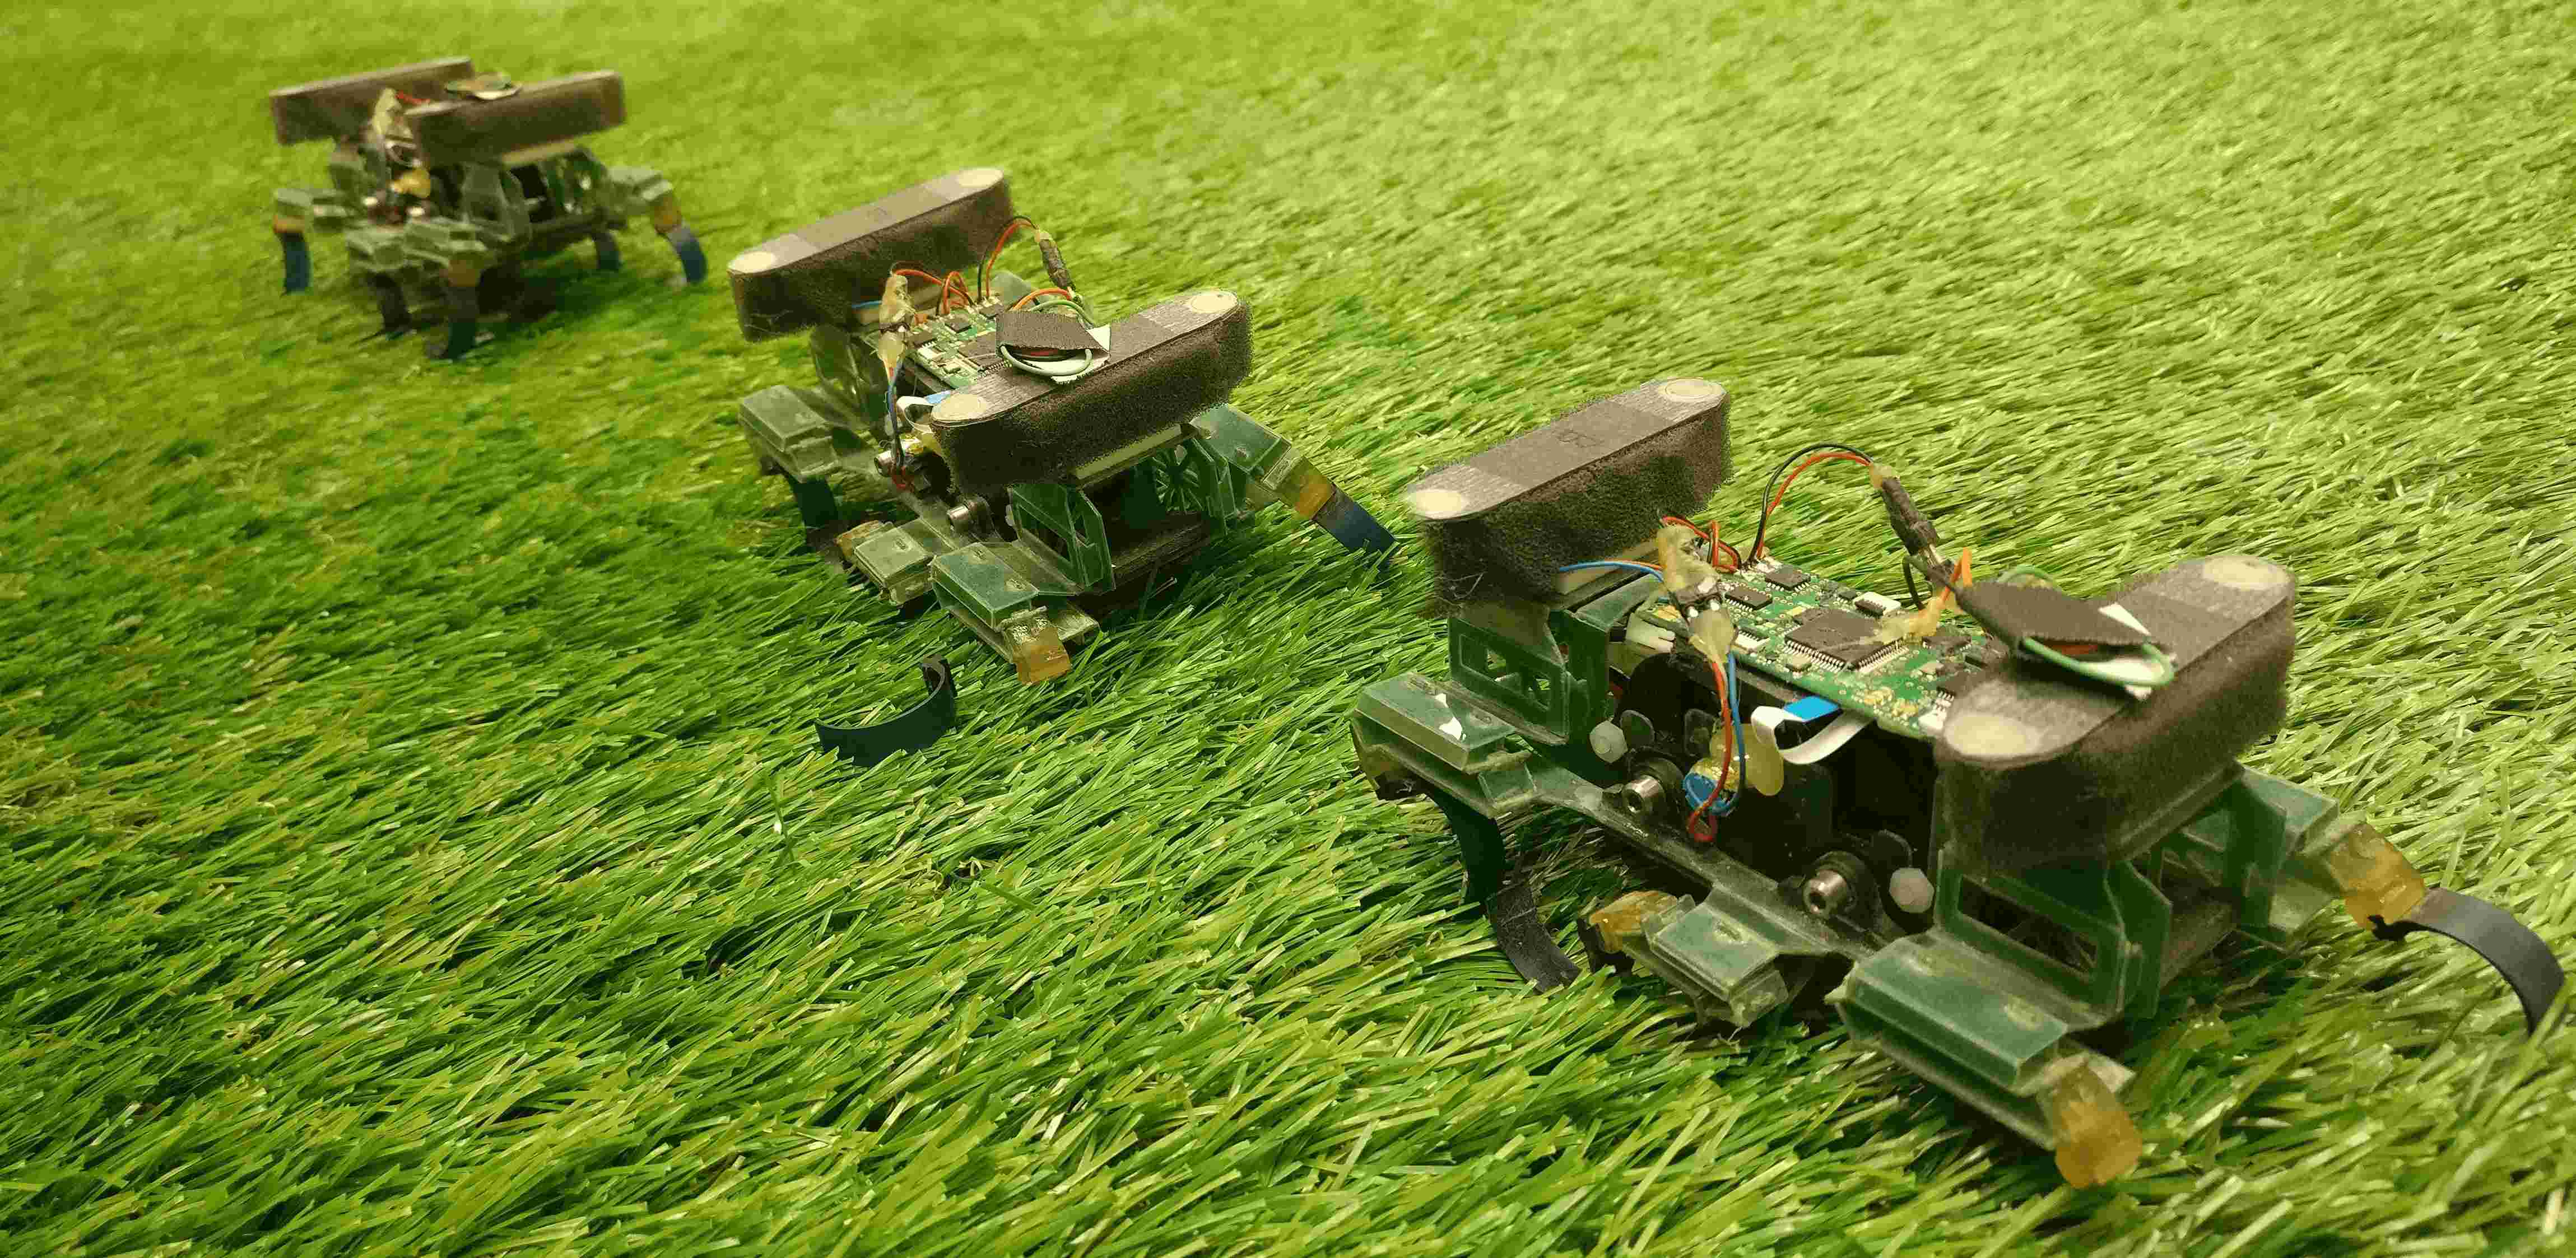
\includegraphics[width=0.55\linewidth, height=0.25\linewidth]
{pictures/roach_adapt/roach_leg_turf_compressed.jpg}
\label{fig:roach_big}
\vspace{-0.1cm}
\caption{\small \footnotesize We implement our sample-efficient meta-reinforcement learning algorithm on a real legged millirobot, enabling online adaptation to new tasks and unexpected occurrences such as losing a leg (shown here), novel terrains and slopes, errors in pose estimation, and pulling payloads.}
\vspace{-0.2in}
\end{figure}